\begin{figure}[t]
    \centering
    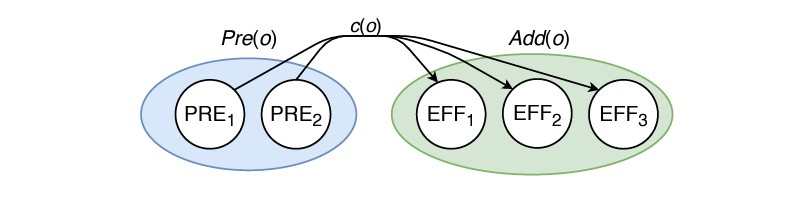
\includegraphics[width=1\textwidth]{figures/images/ch4/nodes_mapping.jpg}
    \caption{Example of nodes and edges definition in \cite{shen2020learning}. The hyper-edge represents an action that connects multiple nodes. The sending nodes are preconditions, while the receiver nodes are the effects.}
    \label{fig:nodes_mapping}
\end{figure}
